\documentclass{article}

% Pakiety wymagane do formatowania i grafiki
\usepackage{geometry}  % Ustawienie marginesów
\usepackage{graphicx}  % Wymagany do wstawiania obrazków
\usepackage{xcolor}    % Kolorowy tekst
\usepackage[T1]{fontenc}
\usepackage[utf8]{inputenc}
\usepackage{polski}
\usepackage{lmodern} 
\usepackage{float}
\usepackage{pgfplots}
\usepackage{titlesec}
\usepackage{multicol}
\usepackage{listings}

\usepackage{fancyhdr} % Pakiet do nagłówków i stopek
\pagestyle{fancy} % Ustawienie niestandardowego stylu


\fancyhead[L]{\includegraphics[width=10cm]{Image/PP-PUT-WORD.png}} % obraz w lewym górnym rogu


\fancyfoot[C]{\thepage}

\usepackage{tcolorbox}
\definecolor{terminalColor}{RGB}{40, 42, 54}
\definecolor{Button1}{RGB}{237, 106, 94}
\definecolor{Button2}{RGB}{245, 191, 79}
\definecolor{Button3}{RGB}{98, 188, 119}



\pgfplotsset{
	width=10cm, height=6cm, ymin=0, xmin=4, xmin=2047, xmax=524288, grid=both, %wymiary osi
	xticklabel style={rotate=45, anchor=near xticklabel},  %liczby na osi X pod kątem 45*
	x label style={at={(axis description cs:0.5,-0.025)}}, %legenda osi X wyśrodkowana, lekko obniżona
}

\renewcommand{\headrulewidth}{0pt} % Usunięcie linii w nagłówku
\renewcommand{\footrulewidth}{0pt} % Cienka linia stopki

% Marginesy strony
\geometry{
	a4paper,
	left=20mm,
	right=20mm,
	top=30mm,
	bottom=25mm,
	headsep=20mm,
}


% Formatowanie sekcji
\titleformat{\section}{\LARGE\bfseries\centering}{}{0em}{}

\begin{document}
	
	\lstset{
		backgroundcolor=\color{black},  % Tło czarne
		basicstyle=\ttfamily\color{white},  % Kolor tekstu biały
		keywordstyle=\color{cyan},  % Kolor słów kluczowych na niebiesko
		commentstyle=\color{gray},  % Kolor komentarzy na szaro
		stringstyle=\color{green},  % Kolor ciągów znaków na zielono
		showstringspaces=false,  % Nie pokazuj spacji w ciągach
		tabsize=3,  % Rozmiar tabulacji
		breaklines=true,  % Łamanie długich linii
		frame=none,  % Bez ramki
		xleftmargin=0cm,  % Margines po lewej stronie
		xrightmargin=0cm,  % Margines po prawej stronie
		aboveskip=0pt,  % Odstęp przed
		belowskip=0pt,  % Odstęp po
		columns=fullflexible,  % Kolumny elastyczne
		linewidth=\linewidth  % Szerokość linii na pełną szerokość
	}
	
	% Strona tytułowa
	\thispagestyle{empty} % Brak nagłówków/stopek na pierwszej stronie
	
	\begin{center}
		\includegraphics[width=6cm]{Image/PP-PUT-LOGO.png}
		\vspace{1cm}
		
		{\Huge\bfseries Politechnika Poznańska}
		
		\vspace{1cm}
		
		{\large Informatyka rok I semestr 2} \\[0.3cm]
		L10, Piątek 11:45 - 13:15
		
		\vspace{1.5cm}
		
		{\LARGE\bfseries Algorytmy i Struktury Danych} \\[0.3cm]
		\textbf{Prowadzący:} Dominik Piotr Witczak
		
		\vspace{2cm}
		
		% Poprawione formatowanie
		{\LARGE\bfseries Sprawozdanie nr 2} 
		
		\vspace{1cm}
		
		{\Large\bfseries Drzewa przeszukiwań binarnych \\
			BST i drzewa samobalansujące AVL}
		
		\vspace{3cm}
		
		\begin{flushright}
			\textbf{Autor:} \\[0.2cm]
			Dominik Fischer 164176 \\
			Oliwer Miller 163544
		\end{flushright}
		
		\vspace{1.5cm}
		Rok akademicki 2024/2025
	\end{center}
	
	
	
	\newpage
	
	\titleformat{\section}{\Huge\bfseries}{\thesection}{2em}{}
	
	\section*{\textcolor{blue}{Wprowadzenie}}
	\noindent Celem niniejszego sprawozdania jest analiza i porównanie dwóch struktur danych: binarnego drzewa poszukiwań BST oraz samobalansującego się drzewa AVL. Obie struktury służą do przechowywania danych w sposób umożliwiający szybkie wyszukiwanie, wstawianie i usuwanie elementów. W praktyce jednak ich wydajność może się znacznie różnić.
	
	\noindent W ramach projektu zaimplementowano oba typy drzew, a następnie dokonano pomiarów czasu wykonywania podstawowych operacji dla zestawów danych o różnej wielkości i strukturze.
	
	\titleformat{\section}{\Large\bfseries}{\thesection}{2em}{}
	\section*{\textcolor{blue}{Tworzenie drzewa BST}}
	\begin{multicols}{2}
		\noindent 
		Klasa \textit{BSTNode} reprezentuje pojedynczy węzeł drzewa BST. Składa się z klucza \textit{key} i odnośników do lewego i prawego potomka. \\ Klasa \textit{BST} reprezentuje drzewo BST. Korzeń drzewa jest zapisany w \textit{root}. Funkcja \textit{insert} służy do dodawania nowych węzłów, wykorzystuje do tego \textit{\_insert}, które rekurencyjnie wstawia węzeł po lewej lub prawej stronie, zależnie od jego wartości. 
		\vspace*{0.4cm}
		\noindent \\Poniżej drzewo BST utworzone z liczb: \\5 8 2 5 10 24 15 11 7 1 2
		\\
		
		\noindent Kolorem czerwonym został zaznaczony korzeń \\
		Kolorem niebieskim węzły wewnętrzne \\
		Kolorem zielonym liście
		
		\vspace*{1cm}
		
		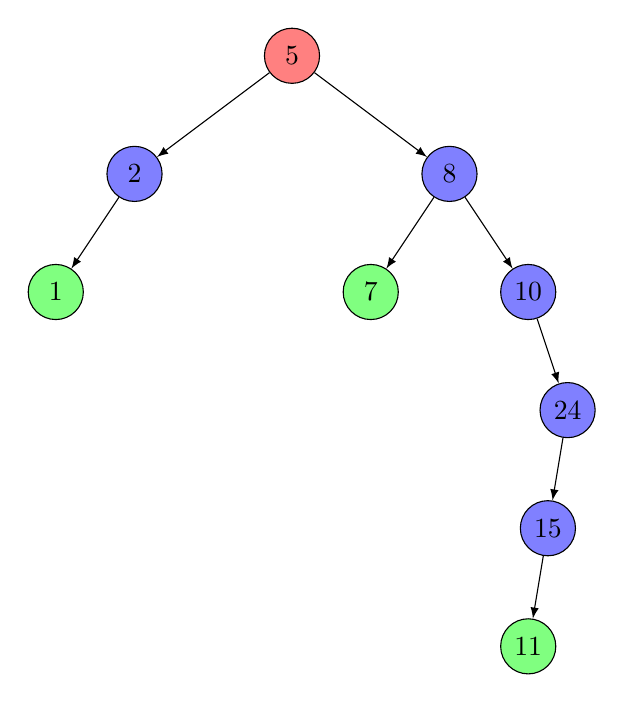
\begin{tikzpicture}[
			grow=down,
			level 1/.style = {sibling distance=4cm},
			level 2/.style = {sibling distance=2cm},
			level 3/.style = {sibling distance=1cm},
			level 4/.style = {sibling distance=0.5cm},
			level distance=1.5cm,
			every node/.style={circle, draw, minimum size=7mm, inner sep=2pt},
			edge from parent/.style={draw, -latex}
			]
			\node[fill=red!50] {5} 
			child { node[fill=blue!50] {2} 
				child { node[fill=green!50] {1} } 
				child [missing] }
			child { node[fill=blue!50] {8} 
				child { node[fill=green!50] {7} } 
				child { node[fill=blue!50] {10} 
					child [missing] 
					child { node[fill=blue!50] {24} 
						child { node[fill=blue!50] {15} 
							child { node[fill=green!50] {11} }
							child [missing] } 
						child [missing] } } };
		\end{tikzpicture} 
		
		\begin{tcolorbox}[colback=black,colframe=gray!50!,arc=3mm,boxrule=0pt,left=0pt,right=0pt,width=\linewidth]
			\textcolor{white}{\textbf{\textsf{Terminal}}}\\
			
			\begin{lstlisting}[language=Python]
class BSTNode:
	def __init__(self, key):
		self.key = key
		self.left = None
		self.right = None

class BST:
	def __init__(self):
		self.root = None

	def insert(self, key):
		self.root = self._insert(self.root, key)

	def _insert(self, node, key):
		if not node:
			return BSTNode(key)
		if key < node.key:
			node.left = self._insert(node.left, key)
		elif key > node.key:
			node.right = self._insert(node.right, key)
		return node
			\end{lstlisting}
			
		\end{tcolorbox}
	\end{multicols}
	
	\newpage
	
	\section*{\textcolor{blue}{Tworzenie drzewa AVL}}
	\begin{multicols}{2}
		\noindent Klasa \textit{AVLNode} ma dodatkowo przypisaną wysokość węzła \textit{height}, wstępnie równa 1, dla przypadku liścia. Przydaje się ona do utrzymania zrównoważenia. \\Funkcja \textit{build\_from\_sorted()} buduje drzewo AVL z posortowanej listy, zgodnie z metodą połowienia binarnego. \\Funkcje \textit{get\_height()} i \textit{update\_height()} mają za zadanie obliczanie i aktualizowanie wysokości węzła, a funkcja \textit{get\_balance()} zwraca współczynnik zrównoważenia. \\Następne są dwie funkcje \textit{rotate\_right} i \textit{rotate\_left} odpowiadające za rotacje w prawo i w lewo, używające wcześniej wspomnianej funkcji \textit{update\_height()}. Funkcja \textit{insert())} jest odpowiedzialna za wstawianie nowego węzła do drzewa. Wykorzystuje do tego \textit{\_insert()} działające rekurencyjnie. Po wstawieniu węzła, aktualizowana jest wysokość i sprawdzany jest balans, w razie potrzeby później mogą zostać wykonane rotacje.\\ \\
		\noindent Poniżej drzewo AVL utworzone z liczb: \\6 2 4 5 3 10 9 8 17 21 20 25 12 11 1 2 \\ \\ 
		\noindent Kolorem czerwonym został zaznaczony korzeń \\
		Kolorem niebieskim węzły wewnętrzne \\
		Kolorem zielonym liście
			
			
		
		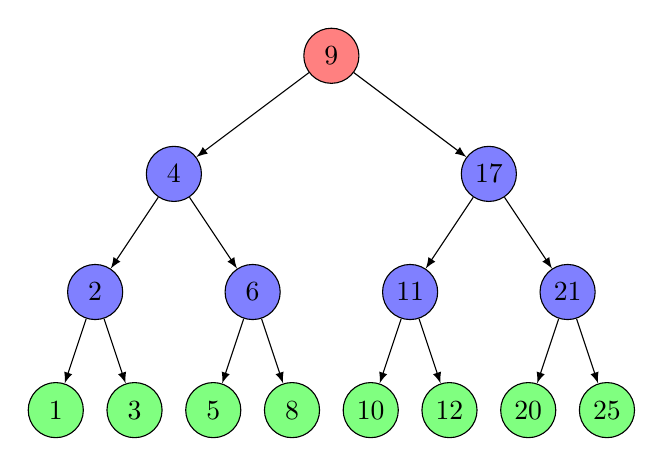
\begin{tikzpicture}[
			grow=down,
			level 1/.style = {sibling distance=4cm},
			level 2/.style = {sibling distance=2cm},
			level 3/.style = {sibling distance=1cm},
			level 4/.style = {sibling distance=0.5cm},
			level distance=1.5cm,
			every node/.style={circle, draw, minimum size=7mm, inner sep=2pt},
			edge from parent/.style={draw, -latex}
			]
			\node[fill=red!50] {9} 
			child { node[fill=blue!50] {4} 
				child { node[fill=blue!50] {2} 
					child { node[fill=green!50] {1} }
					child { node[fill=green!50] {3} } }
				child { node[fill=blue!50] {6} 
					child { node[fill=green!50] {5} }
					child { node[fill=green!50] {8} } } }
			child { node[fill=blue!50] {17} 
				child { node[fill=blue!50] {11} 
					child { node[fill=green!50] {10} }
					child { node[fill=green!50] {12} } }
				child { node[fill=blue!50] {21} 
					child { node[fill=green!50] {20} }
					child { node[fill=green!50] {25} } } };
			\end{tikzpicture}
		\noindent 
		
		\begin{tcolorbox}[colback=black,colframe=gray!50!,arc=3mm,boxrule=0pt,left=0pt,right=0pt,width=\linewidth, sharp corners=south]
			\textcolor{white}{\textbf{\textsf{Terminal}}}\\
			\scriptsize % mniejsza czcionka
			\begin{lstlisting}[language=Python]
class AVLNode:
	def __init__(self, key):
		self.key = key
		self.height = 1
		self.left = None
		self.right = None
	
class AVL:
	def __init__(self):
		self.root = None
	def build_from_sorted(self, values):
		def build(l, r):
			if l > r:
				return None
			mid = (l + r) // 2
			node = AVLNode(values[mid])
			node.left = build(l, mid - 1)
			node.right = build(mid + 1, r)
			node.height = 1 + max(self.get_height(node.left), self.get_height(node.right))
			return node
		self.root = build(0, len(values) - 1)
	def get_height(self, node):
		return node.height if node else 0
	def get_balance(self, node):
		return self.get_height(node.left) - self.get_height(node.right) if node else 0
	def update_height(self, node):
		node.height = 1 + max(self.get_height(node.left), self.get_height(node.right))
	def rotate_right(self, y):
		x = y.left
		T2 = x.right
		x.right = y
		y.left = T2
		self.update_height(y)
		self.update_height(x)
		return x
	def rotate_left(self, x):
		y = x.right
		T2 = y.left
		y.left = x
		x.right = T2
		self.update_height(x)
		self.update_height(y)
		return y
	def insert(self, key):
		self.root = self._insert(self.root, key)
	def _insert(self, node, key):
		if not node:
			return AVLNode(key)
		if key < node.key:
			node.left = self._insert(node.left, key)
		elif key > node.key:
			node.right = self._insert(node.right, key)
		else:
			return node
		self.update_height(node)
		balance = self.get_balance(node)
		if balance > 1 and key < node.left.key:
			return self.rotate_right(node)
		if balance < -1 and key > node.right.key:
			return self.rotate_left(node)
		if balance > 1 and key > node.left.key:
			node.left = self.rotate_left(node.left)
			return self.rotate_right(node)
		if balance < -1 and key < node.right.key:
			node.right = self.rotate_right(node.right)
			return self.rotate_left(node)
		return node
			\end{lstlisting}
		\end{tcolorbox}
	\end{multicols}
	
	\newpage
	\section*{\textcolor{blue}{Porównanie czsów wykonania operacji}}
	
	\begin{figure}[H]
		\centering
		\label{fig:enter-label}
		%Tworzę "pojemnik" na wykres `pgfplots` tak żeby automatycznie wyskalował mi wygenerowany wykres na szerokość strony. 
		\noindent\resizebox{\textwidth}{!}{
			\begin{tikzpicture}
				\begin{axis}[%
					name=plotA, anchor=left of south west,
					title={Tworzenie struktury}, 
					xlabel={Rozmiar instancji}, ylabel={Czas(s)}, legend pos=north west,
					xmode = log, log basis x={2},
					every axis plot post/.style={very thick},
					/tikz/plot label/.style={black, anchor=west}
					]
					\addplot[blue, dashed, smooth] table[x=InputSize,y=Time,meta=Algorithm,col sep=comma] {results/czas_tworzenia_bst.csv};
					\addplot[red, dotted, smooth] table[x=InputSize,y=Time,meta=Algorithm,col sep=comma] {results/czas_tworzenia_avl.csv};
					\legend{BST, AVL}
				\end{axis}
				\begin{axis}[%
					title={Wyszukanie Min/Max}, 
					name=plotB, at=(plotA.right of south east), anchor=left of south west,
					xlabel={Rozmiar instancji}, ylabel={Czas(ms)}, legend pos=north west,
					xmode = log, log basis x={2},
					every axis plot post/.style={very thick},
					/tikz/plot label/.style={black, anchor=west}
					]
					
					\addplot[blue, dashed, smooth] table[x=InputSize,y=Time,meta=Algorithm,col sep=comma] {results/czas_minmax_bst.csv};
					\addplot[red, dotted, smooth] table[x=InputSize,y=Time,meta=Algorithm,col sep=comma] {results/czas_minmax_avl.csv};
					\legend{BST, AVL}
				\end{axis}
				\begin{axis}[%
					title={Równoważenie BST}, 
					name=plotD, at=(plotB.below south west), anchor=above north west,
					xlabel={Rozmiar instancji}, ylabel={Czas(s)}, legend pos=north west,
					xmode = log, log basis x={2},
					every axis plot post/.style={very thick},
					/tikz/plot label/.style={black, anchor=west}
					]
					\addplot[blue, dashed, smooth] table[x=InputSize,y=Time,meta=Algorithm,col sep=comma] {results/czas_balansowania_bst.csv};
					\legend{BST}
				\end{axis}
				\begin{axis}[%
					title={Wypisanie in-order}, 
					name=plotC, at=(plotD.left of south west), anchor=right of south east,
					xlabel={Rozmiar instancji}, ylabel={Czas(s)}, legend pos=north west,
					xmode = log, log basis x={2},
					every axis plot post/.style={very thick},
					/tikz/plot label/.style={black, anchor=west}
					]
					\addplot[blue, dashed, smooth] table[x=InputSize,y=Time,meta=Algorithm,col sep=comma] {results/czas_inorder_bst.csv};
					\addplot[red, dotted, smooth] table[x=InputSize,y=Time,meta=Algorithm,col sep=comma] {results/czas_inorder_avl.csv};
					\legend{BST, AVL}
				\end{axis}
			\end{tikzpicture}
		}
		\caption{Wykresy tworzenia, wyszukania min/max, wypisania in-order, równoważenia}
	\end{figure}
	
\end{document}